% Options for packages loaded elsewhere
\PassOptionsToPackage{unicode}{hyperref}
\PassOptionsToPackage{hyphens}{url}
%
\documentclass[
]{article}
\usepackage{amsmath,amssymb}
\usepackage{lmodern}
\usepackage{iftex}
\ifPDFTeX
  \usepackage[T1]{fontenc}
  \usepackage[utf8]{inputenc}
  \usepackage{textcomp} % provide euro and other symbols
\else % if luatex or xetex
  \usepackage{unicode-math}
  \defaultfontfeatures{Scale=MatchLowercase}
  \defaultfontfeatures[\rmfamily]{Ligatures=TeX,Scale=1}
\fi
% Use upquote if available, for straight quotes in verbatim environments
\IfFileExists{upquote.sty}{\usepackage{upquote}}{}
\IfFileExists{microtype.sty}{% use microtype if available
  \usepackage[]{microtype}
  \UseMicrotypeSet[protrusion]{basicmath} % disable protrusion for tt fonts
}{}
\makeatletter
\@ifundefined{KOMAClassName}{% if non-KOMA class
  \IfFileExists{parskip.sty}{%
    \usepackage{parskip}
  }{% else
    \setlength{\parindent}{0pt}
    \setlength{\parskip}{6pt plus 2pt minus 1pt}}
}{% if KOMA class
  \KOMAoptions{parskip=half}}
\makeatother
\usepackage{xcolor}
\usepackage[margin=1in]{geometry}
\usepackage{color}
\usepackage{fancyvrb}
\newcommand{\VerbBar}{|}
\newcommand{\VERB}{\Verb[commandchars=\\\{\}]}
\DefineVerbatimEnvironment{Highlighting}{Verbatim}{commandchars=\\\{\}}
% Add ',fontsize=\small' for more characters per line
\usepackage{framed}
\definecolor{shadecolor}{RGB}{248,248,248}
\newenvironment{Shaded}{\begin{snugshade}}{\end{snugshade}}
\newcommand{\AlertTok}[1]{\textcolor[rgb]{0.94,0.16,0.16}{#1}}
\newcommand{\AnnotationTok}[1]{\textcolor[rgb]{0.56,0.35,0.01}{\textbf{\textit{#1}}}}
\newcommand{\AttributeTok}[1]{\textcolor[rgb]{0.77,0.63,0.00}{#1}}
\newcommand{\BaseNTok}[1]{\textcolor[rgb]{0.00,0.00,0.81}{#1}}
\newcommand{\BuiltInTok}[1]{#1}
\newcommand{\CharTok}[1]{\textcolor[rgb]{0.31,0.60,0.02}{#1}}
\newcommand{\CommentTok}[1]{\textcolor[rgb]{0.56,0.35,0.01}{\textit{#1}}}
\newcommand{\CommentVarTok}[1]{\textcolor[rgb]{0.56,0.35,0.01}{\textbf{\textit{#1}}}}
\newcommand{\ConstantTok}[1]{\textcolor[rgb]{0.00,0.00,0.00}{#1}}
\newcommand{\ControlFlowTok}[1]{\textcolor[rgb]{0.13,0.29,0.53}{\textbf{#1}}}
\newcommand{\DataTypeTok}[1]{\textcolor[rgb]{0.13,0.29,0.53}{#1}}
\newcommand{\DecValTok}[1]{\textcolor[rgb]{0.00,0.00,0.81}{#1}}
\newcommand{\DocumentationTok}[1]{\textcolor[rgb]{0.56,0.35,0.01}{\textbf{\textit{#1}}}}
\newcommand{\ErrorTok}[1]{\textcolor[rgb]{0.64,0.00,0.00}{\textbf{#1}}}
\newcommand{\ExtensionTok}[1]{#1}
\newcommand{\FloatTok}[1]{\textcolor[rgb]{0.00,0.00,0.81}{#1}}
\newcommand{\FunctionTok}[1]{\textcolor[rgb]{0.00,0.00,0.00}{#1}}
\newcommand{\ImportTok}[1]{#1}
\newcommand{\InformationTok}[1]{\textcolor[rgb]{0.56,0.35,0.01}{\textbf{\textit{#1}}}}
\newcommand{\KeywordTok}[1]{\textcolor[rgb]{0.13,0.29,0.53}{\textbf{#1}}}
\newcommand{\NormalTok}[1]{#1}
\newcommand{\OperatorTok}[1]{\textcolor[rgb]{0.81,0.36,0.00}{\textbf{#1}}}
\newcommand{\OtherTok}[1]{\textcolor[rgb]{0.56,0.35,0.01}{#1}}
\newcommand{\PreprocessorTok}[1]{\textcolor[rgb]{0.56,0.35,0.01}{\textit{#1}}}
\newcommand{\RegionMarkerTok}[1]{#1}
\newcommand{\SpecialCharTok}[1]{\textcolor[rgb]{0.00,0.00,0.00}{#1}}
\newcommand{\SpecialStringTok}[1]{\textcolor[rgb]{0.31,0.60,0.02}{#1}}
\newcommand{\StringTok}[1]{\textcolor[rgb]{0.31,0.60,0.02}{#1}}
\newcommand{\VariableTok}[1]{\textcolor[rgb]{0.00,0.00,0.00}{#1}}
\newcommand{\VerbatimStringTok}[1]{\textcolor[rgb]{0.31,0.60,0.02}{#1}}
\newcommand{\WarningTok}[1]{\textcolor[rgb]{0.56,0.35,0.01}{\textbf{\textit{#1}}}}
\usepackage{graphicx}
\makeatletter
\def\maxwidth{\ifdim\Gin@nat@width>\linewidth\linewidth\else\Gin@nat@width\fi}
\def\maxheight{\ifdim\Gin@nat@height>\textheight\textheight\else\Gin@nat@height\fi}
\makeatother
% Scale images if necessary, so that they will not overflow the page
% margins by default, and it is still possible to overwrite the defaults
% using explicit options in \includegraphics[width, height, ...]{}
\setkeys{Gin}{width=\maxwidth,height=\maxheight,keepaspectratio}
% Set default figure placement to htbp
\makeatletter
\def\fps@figure{htbp}
\makeatother
\setlength{\emergencystretch}{3em} % prevent overfull lines
\providecommand{\tightlist}{%
  \setlength{\itemsep}{0pt}\setlength{\parskip}{0pt}}
\setcounter{secnumdepth}{-\maxdimen} % remove section numbering
\usepackage{statstyle}
\ifLuaTeX
  \usepackage{selnolig}  % disable illegal ligatures
\fi
\IfFileExists{bookmark.sty}{\usepackage{bookmark}}{\usepackage{hyperref}}
\IfFileExists{xurl.sty}{\usepackage{xurl}}{} % add URL line breaks if available
\urlstyle{same} % disable monospaced font for URLs
\hypersetup{
  pdftitle={Simulation study for debiased learning},
  hidelinks,
  pdfcreator={LaTeX via pandoc}}

\title{Simulation study for debiased learning}
\author{}
\date{\vspace{-2.5em}}

\begin{document}
\maketitle

\hypertarget{simulation-setup}{%
\section{Simulation setup}\label{simulation-setup}}

Let \(A\) be a sample of size \(n =\) 500 selected from the population
\(U\) of size \(N =\) 5000. Let \(y\) be a variable of interest and we
try to estimate the population total \(t_y = \sum_{i \in U} y_i\) and
\(\bf x_{i}\) of size \(p\) be the auxiliary variables associated with
\(y\) where \(x_{ij} \iid N(2, 1)\). Suppose the following
superpopulation model holds \[
y_i = \bf x_i^T \bf \beta + \varepsilon_i, \quad \varepsilon_i \iid N(0,\sigma^2), i = 1, \cdots, N
\] where \(\sigma^2 = 1\) and
\(\bf \beta = (1, \cdots, 1, 0, \cdots, 0)\) with \(s =\) 5 1s and
\(p - s =\) 195 0s. We assume the samples are drawn from the SRS
sampling.

We consider the following estimators.

\begin{itemize}
  \item Difference estimator
  $$
  \hat t_y = \pa{\sum_{i \in U}\bf x_i}^T \bf \beta + \sum_{i \in A} d_i \pa{y_i - \bf x_i^T \bf \beta}
  $$
  \item GREG estimator
  $$
  \hat t_y = \pa{\sum_{i \in U}\bf x_i}^T \hat{\bf \beta} + \sum_{i \in A} d_i \pa{y_i - \bf x_i^T \hat{\bf \beta}}
  $$
  where $\hat {\bf \beta} = \pa{\sum_{i \in A} d_i \bf x_i \bf x_i^T}^{-1} \pa{\sum_{i \in A} d_i \bf x_i y_i}$
  
  \item Model-based estimator
  $$
  \hat t_y = \pa{\sum_{i \in U}\bf x_i}^T \hat{\bf \beta}
  $$
  
  \item Debiased GREG estimator(Proposed)
    $$
  \hat t_y = \pa{\sum_{i \in U}\bf x_i}^T \pa{ \frac{\sum_{i \in A_2}d_i}{\sum_{i \in A}d_i} \hat{\bf \beta}_1 + \frac{\sum_{i \in A_1}d_i}{\sum_{i \in A}d_i} \hat{\bf \beta}_2} + \sum_{i \in A_1} d_i \pa{y_i - \bf x_i^T \hat{\bf \beta}_2} + \sum_{i \in A_2} d_i \pa{y_i - \bf x_i^T \hat{\bf \beta}_1}
  $$
  where $A_1$ and $A_2$ are the subsamples of $A$ with $A_1 \bigcup A_2 = A$, and $\hat {\bf \beta}_1$ and $\hat {\bf \beta}_2$ are the regression coefficients built upon the sample $A_1$ and sample $A_2$ respectively.
  \item Design unbiased GREG estimator(Sande, 2021)
  $$
  \hat t_y = \pa{\sum_{i \in U}\bf x_i}^T \hat{\bf \beta}_1 + \sum_{i \in A_1} \pa{y_i - \bf x_i^T \hat{\bf \beta}_1} + \sum_{i \in A_2} \frac{1}{P(i \in A_2 | i \in A)} \pa{y_i - \bf x_i^T \hat{\bf \beta}_1}
  $$
  
  %\item LASSO estimator
  %\item Debiased Lasso estimator(Zhang \& Zhang, 2014)
\end{itemize}

\begin{Shaded}
\begin{Highlighting}[]
\NormalTok{res }\OtherTok{=} \ConstantTok{NULL}
\NormalTok{res2 }\OtherTok{=} \ConstantTok{NULL}
\NormalTok{res3 }\OtherTok{=} \ConstantTok{NULL}
\NormalTok{SIMNUM }\OtherTok{=} \DecValTok{500}
\ControlFlowTok{for}\NormalTok{(simnum }\ControlFlowTok{in} \DecValTok{1}\SpecialCharTok{:}\NormalTok{SIMNUM)\{}
  \FunctionTok{set.seed}\NormalTok{(simnum)}
\NormalTok{  Index }\OtherTok{=} \FunctionTok{sample}\NormalTok{(}\DecValTok{1}\SpecialCharTok{:}\NormalTok{N, }\AttributeTok{size =}\NormalTok{ n, }\AttributeTok{replace =} \ConstantTok{FALSE}\NormalTok{, }\AttributeTok{prob =}\NormalTok{ pi1)}
\NormalTok{y\_s }\OtherTok{=}\NormalTok{ y[Index]}
\NormalTok{X\_s }\OtherTok{=}\NormalTok{ X[Index, ]}
\NormalTok{d1\_s }\OtherTok{=}\NormalTok{ d1[Index]}
\NormalTok{lm\_obj }\OtherTok{=} \FunctionTok{lm}\NormalTok{(y\_s }\SpecialCharTok{\textasciitilde{}}\NormalTok{  X\_s, }\AttributeTok{weights =}\NormalTok{ d1\_s)}
\NormalTok{beta\_hat }\OtherTok{=}\NormalTok{ lm\_obj}\SpecialCharTok{$}\NormalTok{coefficients[}\SpecialCharTok{{-}}\DecValTok{1}\NormalTok{]}
\CommentTok{\#drop(solve(t(X\_s) \%*\% diag(d1\_s) \%*\% X\_s, t(X\_s) \%*\% diag(d1\_s) \%*\% y\_s))}

\CommentTok{\# beta\_hat = unname(lm(y\_s \textasciitilde{}  t(apply(X\_s, 1, function(k) k }
\CommentTok{\# {-} colSums(X\_s * d1\_s) / N)), weights = d1\_s)$coefficients[{-}1])}

\NormalTok{y\_HT }\OtherTok{=} \FunctionTok{sum}\NormalTok{(y\_s }\SpecialCharTok{*}\NormalTok{ d1\_s)}

\NormalTok{y\_diff }\OtherTok{=} \FunctionTok{drop}\NormalTok{(}\FunctionTok{colSums}\NormalTok{(X) }\SpecialCharTok{\%*\%}\NormalTok{ beta }\SpecialCharTok{+} \FunctionTok{sum}\NormalTok{((y\_s }\SpecialCharTok{{-}} \FunctionTok{drop}\NormalTok{(X\_s }\SpecialCharTok{\%*\%}\NormalTok{ beta)) }\SpecialCharTok{*}\NormalTok{ d1\_s))}

\NormalTok{y\_GREG }\OtherTok{=} \FunctionTok{drop}\NormalTok{(}\FunctionTok{colSums}\NormalTok{(X) }\SpecialCharTok{\%*\%}\NormalTok{ beta\_hat }\SpecialCharTok{+} \FunctionTok{sum}\NormalTok{((y\_s }\SpecialCharTok{{-}} \FunctionTok{drop}\NormalTok{(X\_s }\SpecialCharTok{\%*\%}\NormalTok{ beta\_hat)) }\SpecialCharTok{*}\NormalTok{ d1\_s))}

\NormalTok{y\_model }\OtherTok{=} \FunctionTok{drop}\NormalTok{(}\FunctionTok{colSums}\NormalTok{(X) }\SpecialCharTok{\%*\%}\NormalTok{ beta\_hat)}

\NormalTok{Index\_sub1 }\OtherTok{=}\NormalTok{ Index[}\FunctionTok{sample}\NormalTok{(}\DecValTok{1}\SpecialCharTok{:}\NormalTok{n, }\AttributeTok{size =}\NormalTok{ m, }\AttributeTok{replace =} \ConstantTok{FALSE}\NormalTok{)]}
\NormalTok{Index\_sub2 }\OtherTok{=}\NormalTok{ Index[}\SpecialCharTok{!}\NormalTok{(Index }\SpecialCharTok{\%in\%}\NormalTok{ Index\_sub1)]}

\NormalTok{y\_s1 }\OtherTok{=}\NormalTok{ y[Index\_sub1]}
\NormalTok{X\_s1 }\OtherTok{=}\NormalTok{ X[Index\_sub1, ]}
\NormalTok{X1\_s1 }\OtherTok{=} \FunctionTok{cbind}\NormalTok{(}\DecValTok{1}\NormalTok{, X)[Index\_sub1, ]}
\NormalTok{d1\_s1 }\OtherTok{=}\NormalTok{ d1[Index\_sub1]}
\NormalTok{lm\_obj1 }\OtherTok{=} \FunctionTok{lm}\NormalTok{(y\_s1 }\SpecialCharTok{\textasciitilde{}}\NormalTok{  X\_s1, }\AttributeTok{weights =}\NormalTok{ d1\_s1)}
\NormalTok{beta\_hat1 }\OtherTok{=}\NormalTok{ lm\_obj1}\SpecialCharTok{$}\NormalTok{coefficients[}\SpecialCharTok{{-}}\DecValTok{1}\NormalTok{]}

\NormalTok{y\_s2 }\OtherTok{=}\NormalTok{ y[Index\_sub2]}
\NormalTok{X\_s2 }\OtherTok{=}\NormalTok{ X[Index\_sub2, ]}
\NormalTok{d1\_s2 }\OtherTok{=}\NormalTok{ d1[Index\_sub2]}
\NormalTok{lm\_obj2 }\OtherTok{=} \FunctionTok{lm}\NormalTok{(y\_s2 }\SpecialCharTok{\textasciitilde{}}\NormalTok{  X\_s2, }\AttributeTok{weights =}\NormalTok{ d1\_s2)}
\NormalTok{beta\_hat2 }\OtherTok{=}\NormalTok{ lm\_obj2}\SpecialCharTok{$}\NormalTok{coefficients[}\SpecialCharTok{{-}}\DecValTok{1}\NormalTok{]}

\CommentTok{\# y\_debiased = drop(colSums(X) \%*\% beta\_hat + sum((y\_s1 {-} drop(X\_s1 \%*\% beta\_hat2)) * d1\_s1) }
\CommentTok{\# + sum((y\_s2 {-} drop(X\_s2 \%*\% beta\_hat1)) * d1\_s2))}

\NormalTok{y\_debiased }\OtherTok{=} \FunctionTok{drop}\NormalTok{(}\FunctionTok{colSums}\NormalTok{(X) }\SpecialCharTok{\%*\%}\NormalTok{ (}\FunctionTok{sum}\NormalTok{(d1\_s2) }\SpecialCharTok{/} \FunctionTok{sum}\NormalTok{(d1\_s) }\SpecialCharTok{*}\NormalTok{ beta\_hat1 }\SpecialCharTok{+} \FunctionTok{sum}\NormalTok{(d1\_s1) }\SpecialCharTok{/} \FunctionTok{sum}\NormalTok{(d1\_s) }\SpecialCharTok{*}\NormalTok{ beta\_hat2) }\SpecialCharTok{+} 
                    \FunctionTok{sum}\NormalTok{((y\_s1 }\SpecialCharTok{{-}} \FunctionTok{drop}\NormalTok{(X\_s1 }\SpecialCharTok{\%*\%}\NormalTok{ beta\_hat2)) }\SpecialCharTok{*}\NormalTok{ d1\_s1) }\SpecialCharTok{+} \FunctionTok{sum}\NormalTok{((y\_s2 }\SpecialCharTok{{-}} \FunctionTok{drop}\NormalTok{(X\_s2 }\SpecialCharTok{\%*\%}\NormalTok{ beta\_hat1)) }\SpecialCharTok{*}\NormalTok{ d1\_s2))}

\NormalTok{y\_unbiased }\OtherTok{=} \FunctionTok{drop}\NormalTok{(}\FunctionTok{colSums}\NormalTok{(X) }\SpecialCharTok{\%*\%}\NormalTok{ beta\_hat1 }\SpecialCharTok{+} \FunctionTok{sum}\NormalTok{((y\_s1 }\SpecialCharTok{{-}} \FunctionTok{drop}\NormalTok{(X\_s1 }\SpecialCharTok{\%*\%}\NormalTok{ beta\_hat1))) }
                  \SpecialCharTok{+} \FunctionTok{sum}\NormalTok{((y\_s2 }\SpecialCharTok{{-}} \FunctionTok{drop}\NormalTok{(X\_s2 }\SpecialCharTok{\%*\%}\NormalTok{ beta\_hat1)) }\SpecialCharTok{*} \DecValTok{2}\NormalTok{))}

\NormalTok{Omega }\OtherTok{=} \FunctionTok{matrix}\NormalTok{(}\DecValTok{1} \SpecialCharTok{{-}}\NormalTok{ n }\SpecialCharTok{/}\NormalTok{ (n}\DecValTok{{-}1}\NormalTok{) }\SpecialCharTok{*}\NormalTok{ (N}\DecValTok{{-}1}\NormalTok{) }\SpecialCharTok{/}\NormalTok{ N, }\AttributeTok{nr =}\NormalTok{ n, }\AttributeTok{nc =}\NormalTok{ n)}
\FunctionTok{diag}\NormalTok{(Omega) }\OtherTok{=} \DecValTok{1} \SpecialCharTok{{-}}\NormalTok{ n }\SpecialCharTok{/}\NormalTok{ N}


\NormalTok{e\_s }\OtherTok{=}\NormalTok{ y\_s }\SpecialCharTok{{-}}\NormalTok{ X\_s }\SpecialCharTok{\%*\%}\NormalTok{ beta}
\NormalTok{sigma\_diff }\OtherTok{=} \FunctionTok{sqrt}\NormalTok{(}\FunctionTok{drop}\NormalTok{(}\FunctionTok{t}\NormalTok{(e\_s)  }\SpecialCharTok{\%*\%}\NormalTok{ Omega }\SpecialCharTok{\%*\%}\NormalTok{ e\_s }\SpecialCharTok{*}\NormalTok{ N}\SpecialCharTok{\^{}}\DecValTok{2} \SpecialCharTok{/}\NormalTok{ n}\SpecialCharTok{\^{}}\DecValTok{2}\NormalTok{))}

\CommentTok{\# sum(sapply(1:n, function(k) sapply(1:n, function(l) }
\CommentTok{\#   ifelse(k == l, 1 {-} n / N, 1 {-} n / (n {-} 1) * (N {-} 1) / N) * e\_s[k] * e\_s[l] * N / n * N / n  ))) / N\^{}2}

\NormalTok{e\_s }\OtherTok{=}\NormalTok{ y\_s }\SpecialCharTok{{-}}\NormalTok{ X\_s }\SpecialCharTok{\%*\%}\NormalTok{ beta\_hat}
\NormalTok{sigma\_GREG }\OtherTok{=} \FunctionTok{sqrt}\NormalTok{(}\FunctionTok{drop}\NormalTok{(}\FunctionTok{t}\NormalTok{(e\_s)  }\SpecialCharTok{\%*\%}\NormalTok{ Omega }\SpecialCharTok{\%*\%}\NormalTok{ e\_s }\SpecialCharTok{*}\NormalTok{ N}\SpecialCharTok{\^{}}\DecValTok{2} \SpecialCharTok{/}\NormalTok{ n}\SpecialCharTok{\^{}}\DecValTok{2}\NormalTok{))}

\CommentTok{\# e\_s = ifelse(Index \%in\% Index\_sub1, y\_s {-} X\_s \%*\% beta\_hat2, y\_s {-} X\_s \%*\% beta\_hat1)}
\CommentTok{\# \# e\_s = ifelse(Index \%in\% Index\_sub1, y\_s {-} X\_s \%*\% beta\_hat1, y\_s {-} X\_s \%*\% beta\_hat2)}
\CommentTok{\# \# e\_s = c(y\_s1 {-} X\_s1 \%*\% beta\_hat2, y\_s2 {-} X\_s2 \%*\% beta\_hat1)}
\CommentTok{\# sigma\_Debiased = sqrt(drop(t(e\_s)  \%*\% Omega \%*\% e\_s * N\^{}2 / n\^{}2))}

\NormalTok{e\_s1 }\OtherTok{=} \FunctionTok{ifelse}\NormalTok{(Index }\SpecialCharTok{\%in\%}\NormalTok{ Index\_sub1, y\_s }\SpecialCharTok{{-}}\NormalTok{ X\_s }\SpecialCharTok{\%*\%}\NormalTok{ beta\_hat1, }\DecValTok{0}\NormalTok{)}
\NormalTok{e\_s2 }\OtherTok{=} \FunctionTok{ifelse}\NormalTok{(Index }\SpecialCharTok{\%in\%}\NormalTok{ Index\_sub2, y\_s }\SpecialCharTok{{-}}\NormalTok{ X\_s }\SpecialCharTok{\%*\%}\NormalTok{ beta\_hat2, }\DecValTok{0}\NormalTok{)}

\NormalTok{sigma\_Debiased }\OtherTok{=} \FunctionTok{sqrt}\NormalTok{(}\FunctionTok{drop}\NormalTok{((}\FunctionTok{t}\NormalTok{(e\_s1)  }\SpecialCharTok{\%*\%}\NormalTok{ Omega }\SpecialCharTok{\%*\%}\NormalTok{ e\_s1 }\SpecialCharTok{+} \FunctionTok{t}\NormalTok{(e\_s2)  }\SpecialCharTok{\%*\%}\NormalTok{ Omega }\SpecialCharTok{\%*\%}\NormalTok{ e\_s2) }\SpecialCharTok{*}\NormalTok{ N}\SpecialCharTok{\^{}}\DecValTok{2} \SpecialCharTok{/}\NormalTok{ n}\SpecialCharTok{\^{}}\DecValTok{2}\NormalTok{))}

\NormalTok{res }\OtherTok{=} \FunctionTok{rbind}\NormalTok{(res, }\FunctionTok{c}\NormalTok{(}\AttributeTok{Diff =}\NormalTok{ y\_diff, }\AttributeTok{GREG =}\NormalTok{ y\_GREG, }\AttributeTok{Model =}\NormalTok{ y\_model, }\AttributeTok{Debiased =}\NormalTok{ y\_debiased, }\AttributeTok{Unbiased =}\NormalTok{ y\_unbiased, }\AttributeTok{HT =}\NormalTok{ y\_HT))}

\NormalTok{res2 }\OtherTok{=} \FunctionTok{rbind}\NormalTok{(res2, }\FunctionTok{c}\NormalTok{(}\AttributeTok{Diff =}\NormalTok{ sigma\_diff, }\AttributeTok{GREG =}\NormalTok{ sigma\_GREG, }\AttributeTok{Debiased =}\NormalTok{ sigma\_Debiased))}

\CommentTok{\# res3 = rbind(res3, c(sum((y\_s1 {-} drop(X\_s1 \%*\% beta\_hat2)) * d1\_s1), sum((y\_s2 {-} drop(X\_s2 \%*\% beta\_hat1)) * d1\_s2)))}

\NormalTok{res3 }\OtherTok{=} \FunctionTok{rbind}\NormalTok{(res3, }\FunctionTok{c}\NormalTok{(}\FunctionTok{colMeans}\NormalTok{(X\_s), beta\_hat))}

\NormalTok{\}}

\NormalTok{BIAS }\OtherTok{=} \FunctionTok{colMeans}\NormalTok{(res }\SpecialCharTok{{-}}\NormalTok{ t\_y)}
\NormalTok{SE }\OtherTok{=} \FunctionTok{apply}\NormalTok{(res, }\DecValTok{2}\NormalTok{, }\ControlFlowTok{function}\NormalTok{(x) }\FunctionTok{sqrt}\NormalTok{(}\FunctionTok{var}\NormalTok{(x) }\SpecialCharTok{*}\NormalTok{ (}\FunctionTok{length}\NormalTok{(x)}\SpecialCharTok{{-}}\DecValTok{1}\NormalTok{)}\SpecialCharTok{/}\FunctionTok{length}\NormalTok{(x) ))}
\NormalTok{RMSE }\OtherTok{=} \FunctionTok{apply}\NormalTok{(res }\SpecialCharTok{{-}}\NormalTok{ t\_y, }\DecValTok{2}\NormalTok{, }\ControlFlowTok{function}\NormalTok{(x) }\FunctionTok{sqrt}\NormalTok{(}\FunctionTok{mean}\NormalTok{(x}\SpecialCharTok{\^{}}\DecValTok{2}\NormalTok{)))}

\FunctionTok{cbind}\NormalTok{(BIAS, SE, RMSE)}
\end{Highlighting}
\end{Shaded}

\begin{verbatim}
##                  BIAS         SE       RMSE
## Diff        22.493403   220.9426   222.0847
## GREG        27.427755   274.4130   275.7803
## Model    -2755.787515  7829.9093  8300.7135
## Debiased    17.064931   502.7975   503.0870
## Unbiased -3496.489480 16786.8144 17147.0865
## HT           9.820459   543.7638   543.8525
\end{verbatim}

\hypertarget{variance-estimation}{%
\section{Variance estimation}\label{variance-estimation}}

Consider the following variance estimation method for estimating the
variance of debiased estimator: \[
V_p\pa{\sum_{i \in A_1}\frac{y_i - \bf x_i \hat {\bf \beta}_2}{\pi_i}} + V_p\pa{\sum_{i \in A_2}\frac{y_i - \bf x_i \hat {\bf \beta}_1}{\pi_i}}
\]

\begin{Shaded}
\begin{Highlighting}[]
\NormalTok{BIAS2 }\OtherTok{=} \FunctionTok{colMeans}\NormalTok{(res2 }\SpecialCharTok{{-}} \FunctionTok{rep}\NormalTok{(SE[}\FunctionTok{c}\NormalTok{(}\DecValTok{1}\NormalTok{,}\DecValTok{2}\NormalTok{,}\DecValTok{4}\NormalTok{)], }\AttributeTok{each =}\NormalTok{ SIMNUM))}
\NormalTok{SE2 }\OtherTok{=} \FunctionTok{apply}\NormalTok{(res2, }\DecValTok{2}\NormalTok{, }\ControlFlowTok{function}\NormalTok{(x) }\FunctionTok{sqrt}\NormalTok{(}\FunctionTok{var}\NormalTok{(x) }\SpecialCharTok{*}\NormalTok{ (}\FunctionTok{length}\NormalTok{(x)}\SpecialCharTok{{-}}\DecValTok{1}\NormalTok{)}\SpecialCharTok{/}\FunctionTok{length}\NormalTok{(x) ))}
\NormalTok{RMSE2 }\OtherTok{=} \FunctionTok{apply}\NormalTok{(res2 }\SpecialCharTok{{-}} \FunctionTok{rep}\NormalTok{(SE[}\FunctionTok{c}\NormalTok{(}\DecValTok{1}\NormalTok{,}\DecValTok{2}\NormalTok{,}\DecValTok{4}\NormalTok{)], }\AttributeTok{each =}\NormalTok{ SIMNUM), }\DecValTok{2}\NormalTok{, }\ControlFlowTok{function}\NormalTok{(x) }\FunctionTok{sqrt}\NormalTok{(}\FunctionTok{mean}\NormalTok{(x}\SpecialCharTok{\^{}}\DecValTok{2}\NormalTok{)))}
\NormalTok{MidErr2 }\OtherTok{=} \FunctionTok{apply}\NormalTok{(res2 }\SpecialCharTok{{-}} \FunctionTok{rep}\NormalTok{(SE[}\FunctionTok{c}\NormalTok{(}\DecValTok{1}\NormalTok{,}\DecValTok{2}\NormalTok{,}\DecValTok{4}\NormalTok{)], }\AttributeTok{each =}\NormalTok{ SIMNUM), }\DecValTok{2}\NormalTok{, median)}

\FunctionTok{cbind}\NormalTok{(BIAS2, SE2, RMSE2, MidErr2)}
\end{Highlighting}
\end{Shaded}

\begin{verbatim}
##                BIAS2       SE2    RMSE2    MidErr2
## Diff       -9.977691   6.62237  11.9754  -10.10267
## GREG     -111.126214   6.64782 111.3249 -111.63912
## Debiased   48.174842 267.71327 272.0133   22.11643
\end{verbatim}

\begin{Shaded}
\begin{Highlighting}[]
\FunctionTok{plot}\NormalTok{(res2[,}\DecValTok{2}\NormalTok{], }\AttributeTok{main =} \StringTok{"GREG"}\NormalTok{, }\AttributeTok{ylim =} \FunctionTok{c}\NormalTok{(}\FunctionTok{min}\NormalTok{(res2[,}\DecValTok{2}\NormalTok{]), SE[}\DecValTok{2}\NormalTok{]))}
\FunctionTok{abline}\NormalTok{(}\AttributeTok{h =}\NormalTok{ SE[}\DecValTok{2}\NormalTok{], }\AttributeTok{col =} \StringTok{"blue"}\NormalTok{)}
\FunctionTok{abline}\NormalTok{(}\AttributeTok{h =} \FunctionTok{median}\NormalTok{(res2[,}\DecValTok{2}\NormalTok{]), }\AttributeTok{col =} \StringTok{"red"}\NormalTok{)}
\end{Highlighting}
\end{Shaded}


\includegraphics{sim_files/figure-latex/unnamed-chunk-3-1.pdf}

\begin{Shaded}
\begin{Highlighting}[]
\FunctionTok{plot}\NormalTok{(res2[,}\DecValTok{3}\NormalTok{], }\AttributeTok{main =} \StringTok{"Debiased"}\NormalTok{)}
\FunctionTok{abline}\NormalTok{(}\AttributeTok{h =}\NormalTok{ SE[}\DecValTok{4}\NormalTok{], }\AttributeTok{col =} \StringTok{"blue"}\NormalTok{)}
\FunctionTok{abline}\NormalTok{(}\AttributeTok{h =} \FunctionTok{median}\NormalTok{(res2[,}\DecValTok{3}\NormalTok{]), }\AttributeTok{col =} \StringTok{"red"}\NormalTok{)}
\end{Highlighting}
\end{Shaded}

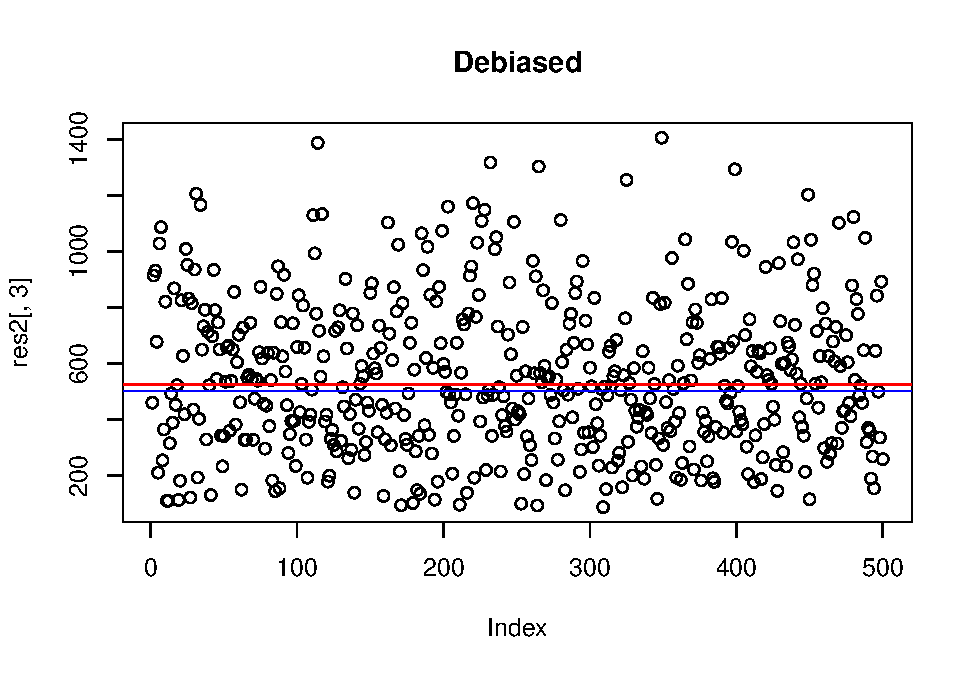
\includegraphics{sim_files/figure-latex/unnamed-chunk-4-1.pdf}

\begin{Shaded}
\begin{Highlighting}[]
\CommentTok{\# median(res2[,3])}
\end{Highlighting}
\end{Shaded}

\begin{Shaded}
\begin{Highlighting}[]
\FunctionTok{hist}\NormalTok{(res2[,}\DecValTok{3}\NormalTok{], }\AttributeTok{main =} \StringTok{"SE of Debiased estimator"}\NormalTok{)}
\end{Highlighting}
\end{Shaded}

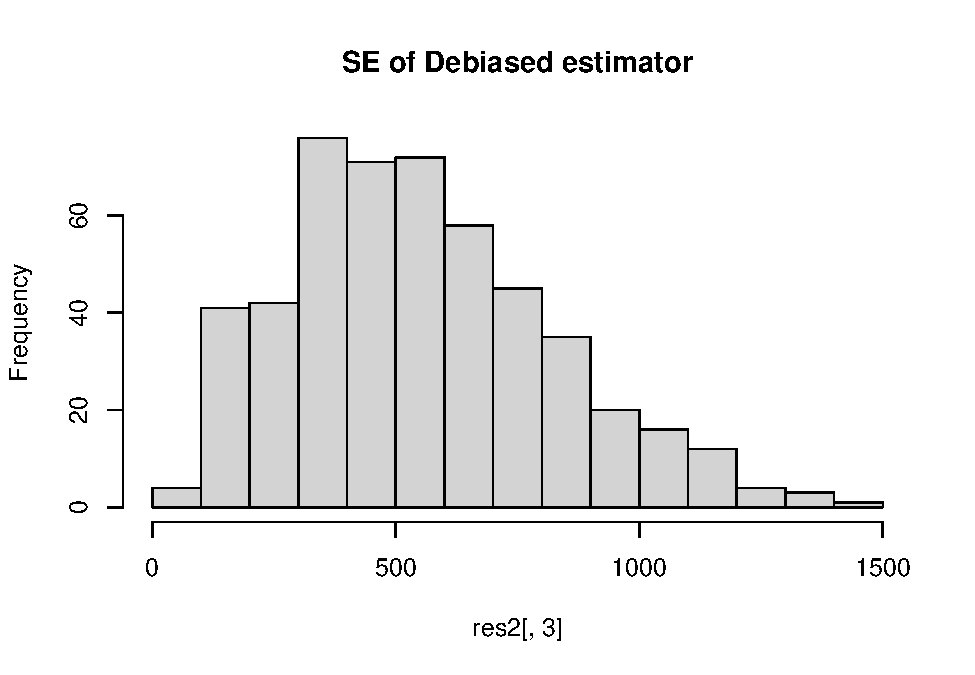
\includegraphics{sim_files/figure-latex/unnamed-chunk-5-1.pdf}

\end{document}
